\documentclass[11 pt]{article}

\usepackage{graphicx}

\usepackage{setspace}
\setstretch{1.25}

\begin{document}  
  \begin{titlepage}
\begin{center}
\huge{\bfseries{System Testing:}}\\
[2mm]
\huge{\bfseries{Prime Number Function}}\\
Version 1.0\\
  \vskip 0.2in
 Prince Ngema (754774)\\
 Tholithemba Mngomezulu (1512124)\\
 Luyanda Makhoba (834867) \\
 Takatso Molekane (569869)\\
 
 

\end{center}
 \end{titlepage}
 \tableofcontents
 \newpage
\subsection{Test Program Description}

\subsection{Screnarios tested and results}
\begin{tabular}{|p{3cm}|p{9cm}|}
\hline
\textbf{Term} & \textbf{Definition}\\
\hline
DCMS &  A Dental Clinic Management System application\\
\hline
User &  Anyone who will be interacting directly with the system..\\
\hline
Netbeans & an integrated development environment for java\\
\hline
Java & A general-purpose computer-programming language that is concurrent, class-based,object-oriented\\
\hline
PHP & Hypertext Preprocessor is a server-side scripting language designed for web development. \\
\hline
Json & JavaScript Object Notation is an open-standard file format that uses human readable text to transmit data objects consisting of attribute-value pairs and array data types \\
\hline
\end{tabular}

    \begin{figure}[h]
    \centering
    
    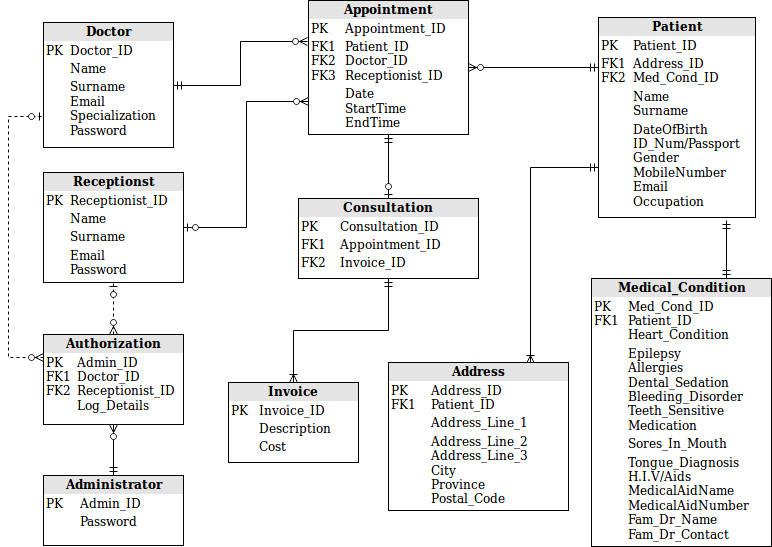
\includegraphics[width=\linewidth]{Dentist ERD.png}
    \caption{DCMS-ERD}
    \label{fig:ERD}
    \end{figure}
 
    
 \end{document}


